% !TEX TS-program = pdflatex
% !TEX encoding = UTF-8 Unicode

% This is a simple template for a LaTeX document using the "article" class.
% See "book", "report", "letter" for other types of document.

\documentclass[11pt]{article} % use larger type; default would be 10pt

\usepackage[utf8]{inputenc} % set input encoding (not needed with XeLaTeX)
\usepackage[backend=biber, style=authoryear]{biblatex}
\addbibresource{bibliography.bib}
%%% Examples of Article customizations
% These packages are optional, depending whether you want the features they provide.
% See the LaTeX Companion or other references for full information.

%%% PAGE DIMENSIONS
\usepackage{geometry} % to change the page dimensions
\geometry{a4paper} % or letterpaper (US) or a5paper or....
% \geometry{margin=2in} % for example, change the margins to 2 inches all round
% \geometry{landscape} % set up the page for landscape
%   read geometry.pdf for detailed page layout information

%\usepackage{graphicx} % support the \includegraphics command and options

\usepackage[parfill]{parskip} % Activate to begin paragraphs with an empty line rather than an indent

%%% PACKAGES
\usepackage{rotating}
\usepackage{booktabs} % for much better looking tables
\usepackage{array} % for better arrays (eg matrices) in maths
\usepackage{paralist} % very flexible & customisable lists (eg. enumerate/itemize, etc.)
\usepackage{verbatim} % adds environment for commenting out blocks of text & for better verbatim
\usepackage{subfig} % make it possible to include more than one captioned figure/table in a single float
\usepackage{graphicx}
\usepackage{csvsimple}
% These packages are all incorporated in the memoir class to one degree or another...

%%% HEADERS & FOOTERS
\usepackage{fancyhdr} % This should be set AFTER setting up the page geometry
\pagestyle{fancy} % options: empty , plain , fancy
\renewcommand{\headrulewidth}{0pt} % customise the layout...
\lhead{}\chead{}\rhead{}
\lfoot{}\cfoot{\thepage}\rfoot{}

%%% SECTION TITLE APPEARANCE
\usepackage{sectsty}
\allsectionsfont{\sffamily\mdseries\upshape} % (See the fntguide.pdf for font help)
% (This matches ConTeXt defaults)

%%% ToC (table of contents) APPEARANCE
\usepackage[nottoc,notlof,notlot]{tocbibind} % Put the bibliography in the ToC
\usepackage[titles,subfigure]{tocloft} % Alter the style of the Table of Contents
\renewcommand{\cftsecfont}{\rmfamily\mdseries\upshape}
\renewcommand{\cftsecpagefont}{\rmfamily\mdseries\upshape} % No bold!

%%% END Article customizations

%%% The "real" document content comes below...

\title{\vspace{-3.0cm}Urban Simulation Assessment}
%\date{} % Activate to display a given date or no date (if empty),
         % otherwise the current date is printed 

\begin{document}
\maketitle


3103 words excluding equations, code, headings, tables, and figures

%%%%%%%%%%%%%%%%%%%%%%%%%%%%%%%%%%%%%%%%%%%%%%%%%%%%%%%%%%%%%%%%%%%%%

\section{Part 1}

% to combine each part into one overall repo for the submission. ended up just adding all the files to a new repo bc it didn't look like the procedure was compatible with github

% in hindsight, I probably could have forked the Main repo, added the files from another part and merged twice. Would that have been better? 
% https://saintgimp.org/2013/01/22/merging-two-git-repositories-into-one-repository-without-losing-file-history/

\subsection{Introduction}

This analysis uses a recursive function for node removal to calculate the marginal effect of a node's removal to consider the resilience of London's tube. Appendix 1 contains code for the function. Below, criteria for node removal and effect evaluation are discussed. 


\subsection{Impact Evaluation}
The network effect metric will be discussed first because the node removal criteria was decided in the context of the network metric.

Breaking the network into isolates was investigated but not pursued. Instead, the focus will be on increasing the total length of a journey. 

This is investigated using shortest topological path. Given the spatial nature of the tubes, where edge attributes represent actual distances, weighted shortest path might be an attractive option. In the context of the London tube though, total time and effort are more important than total distance. Trains can travel longer distances fairly rapidly while traveling through a high number of stations increases time because of the need to stop. Further, it is assumed that traveling through a higher number of stops implies a higher number of train changes which are difficult and slow. Thus by using geodesic path, what is being maximized is the increase in stoppage time, and line change time for travelers in the network.

The igraph package's \verb!mean_distance()! function computes the average shortest path between nodes in the network. The unconnected parameter was used to specify that nodes that were not connected to the largest cluster were counted as 1 + the longest possible geodesic, the actual longest geodesic is much less than this. This demonstrates the incompatibility of different network measures. There was not a clear method for comparing the effect of a longer trip with the effect of removing a trip possibility entirely. 

\subsection{Node Removal Criteria}

For each node, degree, betweeness, topological betweenness, closeness, topological closeness and eigenvector centrality were calculated. The correlations for these values across stations can be reviewed in figure 1. It was noted that correlations between weighted and topological measures were high, indicating that the distances between tube stations are fairly consistent This supports the decision to use geodesic longest path. The correlation of measures betweenness and degree is also fairly high, indicating that tube stations at the middle of a line, with higher betweenness, also tend to have multiple lines, high degree. Correlations between eigenvector centrality and the other measures was very low, indicating that this does not give the same information as other metrics. Lastly, it was not clear why correlation between weighted and topological eigenvector centrality was 0.

In order to maximize the increase in travel time measured by the average length of geodesic paths, betweenness will be used to order node removals. This measure is the number of shortest paths between nodes that travel through a given node. Deleting the node with highest betweenness will force the highest number of trips to use an alternate, longer, path.  

% correlation

\begin{figure}
\centering
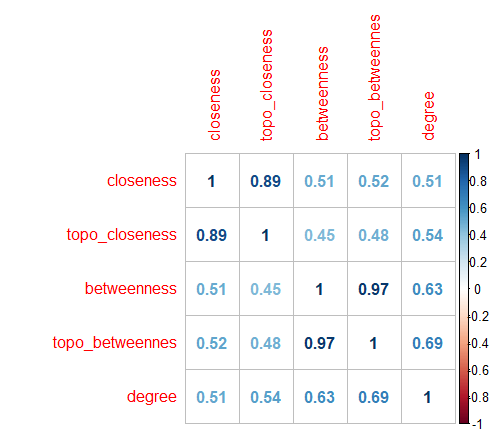
\includegraphics[width=0.8\textwidth]{cropped_correlations}
\caption{Correlation between station/node metrics}
\end{figure}

%
%\begin{center}
%\csvautotabular{betfalse.csv}
%\end{center}

\begin{table}[htbp]
\centering
\begin{tabular}{|r|l|r|r|}
\hline
\multicolumn{1}{|l|}{} & Node Deleted & \multicolumn{1}{l|}{$\Delta$ Avg Geodesic} & \multicolumn{1}{l|}{Components} \\ \hline
1 & Green Park & 0.46 & 1 \\ 
2 & King's Cross St. Pancras & 30.97 & 2 \\ 
3 & Bank & 1.01 & 2 \\ 
4 & Waterloo & 1.14 & 2 \\ 
5 & Stockwell & 17.73 & 4 \\ 
6 & Embankment & 108.62 & 5 \\ 
7 & Baker Street & 2.77 & 6 \\ 
8 & Notting Hill Gate & 30.67 & 7 \\ 
9 & Ealing Common & 26.62 & 9 \\ 
10 & Stratford & 10.58 & 10 \\ 
11 & Canning Town & 5.34 & 12 \\ 
12 & Hammersmith & 8.38 & 14 \\ 
13 & Shadwell & 7.83 & 16 \\ 
14 & Harrow-on-the-Hill & 2.89 & 18 \\ 
15 & Camden Town & 2.38 & 20 \\ 
16 & Canary Wharf & 1.96 & 23 \\ 
17 & Mile End & 0.96 & 24 \\ 
18 & Paddington & 0.18 & 28 \\ 
19 & Earl's Court & 0.11 & 31 \\ 
20 & Oxford Circus & -0.44 & 33 \\ 
21 & Woodford & -0.43 & 34 \\ 
22 & Aldgate East & -0.63 & 35 \\ 
23 & Finsbury Park & -0.35 & 38 \\ 
24 & Northfields & -0.42 & 39 \\ 
25 & Wembley Park & -0.54 & 41 \\ 
26 & North Acton & -0.59 & 43 \\ 
27 & Upney & -0.59 & 44 \\ 
28 & Rayners Lane & -0.60 & 46 \\ 
29 & Liverpool Street & -0.60 & 48 \\ 
30 & London Bridge & -0.60 & 50 \\ \hline
\end{tabular}
\caption{Network effect of prioritizing removal by betweenness \\ (unnconnected = false)}
\label{betweenness false}
\end{table}

% betweenness unconn is true

\begin{table}[htbp]
\centering
\begin{tabular}{|l|r|r|}
\hline
Node Deleted & \multicolumn{1}{l|}{$\Delta$ Avg Geodesic} & \multicolumn{1}{l|}{Components} \\ \hline
Green Park & 0.46 & 1 \\ 
King's Cross St. Pancras & 0.34 & 2 \\ 
Bank & 1.14 & 2 \\ 
Waterloo & 1.28 & 2 \\ 
Stockwell & 0.56 & 4 \\ 
Embankment & -6.17 & 5 \\ 
Baker Street & 2.32 & 6 \\ 
Notting Hill Gate & -1.74 & 7 \\ 
Ealing Common & -2.86 & 9 \\ 
Stratford & -0.36 & 10 \\ 
Canning Town & 0.34 & 12 \\ 
Hammersmith & -1.11 & 14 \\ 
Shadwell & -1.44 & 16 \\ 
Harrow-on-the-Hill & -0.49 & 18 \\ 
Camden Town & -0.57 & 20 \\ 
Canary Wharf & -0.34 & 23 \\ 
Mile End & -0.85 & 24 \\ 
Paddington & -0.33 & 28 \\ 
Earl's Court & -0.20 & 31 \\ 
Oxford Circus & 0.02 & 33 \\ 
Woodford & -0.06 & 34 \\ 
Aldgate East & 0.00 & 35 \\ 
Finsbury Park & -0.10 & 38 \\ 
Northfields & -0.21 & 39 \\ 
Wembley Park & 0.01 & 41 \\ 
North Acton & -0.08 & 43 \\ 
Upney & -0.18 & 44 \\ 
Rayners Lane & -0.12 & 46 \\ 
Liverpool Street & -0.10 & 48 \\ 
London Bridge & -0.08 & 50 \\ \hline
\end{tabular}
\caption{Network effect of prioritizing by betweenness \\ (unnconnected = true)}
\label{betweenness true}
\end{table}

% eigenvector centality, uncon is false

\begin{table}[htbp]
\centering
\begin{tabular}{|r|l|r|r|}
\hline
\multicolumn{1}{|l|}{} & Node Deleted & \multicolumn{1}{l|}{$\Delta$ Avg Geodesic} & \multicolumn{1}{l|}{Components} \\ \hline
1 & Embankment & 0.12 & 1 \\ 
2 & Cannon Street & 5.66 & 2 \\ 
3 & Moorgate & 0.22 & 2 \\ 
4 & West India Quay & 0.02 & 2 \\ 
5 & Great Portland Street & 0.11 & 2 \\ 
6 & Farringdon & 1.91 & 3 \\ 
7 & Paddington & 23.34 & 4 \\ 
8 & Leicester Square & 0.02 & 4 \\ 
9 & Heron Quays & 15.48 & 5 \\ 
10 & Gloucester Road & 0.32 & 5 \\ 
11 & Euston & 34.93 & 6 \\ 
12 & Aldgate & -0.03 & 6 \\ 
13 & St. James's Park & -0.02 & 6 \\ 
14 & Mile End & 0.50 & 6 \\ 
15 & Oxford Circus & 0.31 & 6 \\ 
16 & Notting Hill Gate & 3.48 & 7 \\ 
17 & Rotherhithe & -0.02 & 7 \\ 
18 & Blackfriars & -1.59 & 8 \\ 
19 & Baker Street & 90.79 & 12 \\ 
20 & Barons Court & 5.84 & 13 \\ 
21 & Aldgate East & 1.50 & 14 \\ 
22 & Ruislip Manor & 1.33 & 15 \\ 
23 & Blackwall & -0.34 & 15 \\ 
24 & King's Cross St. Pancras & 15.42 & 18 \\ 
25 & Island Gardens & -1.07 & 19 \\ 
26 & West Ham & 9.42 & 21 \\ 
27 & Holborn & 2.77 & 24 \\ 
28 & Waterloo & -0.37 & 24 \\ 
29 & Victoria & 5.98 & 25 \\ 
30 & Custom House & 2.37 & 26 \\ \hline
\end{tabular}
\caption{Network effect of prioritizing  by eigenvector centrality \\ (unnconnected = false)}
\label{eig true}
\end{table}

% eigenvector centrality uncon is true. 

\begin{table}[htbp]
\centering
\begin{tabular}{|r|l|r|r|}
\hline
\multicolumn{1}{|l|}{} & Node Deleted & \multicolumn{1}{l|}{$\Delta$ Avg Geodesic} & \multicolumn{1}{l|}{Components} \\ \hline
1 & Embankment & 0.12 & 1 \\ 
2 & Cannon Street & -0.02 & 2 \\ 
3 & Moorgate & 0.22 & 2 \\ 
4 & West India Quay & 0.02 & 2 \\ 
5 & Great Portland Street & 0.11 & 2 \\ 
6 & Farringdon & 0.03 & 3 \\ 
7 & Paddington & -0.07 & 4 \\ 
8 & Leicester Square & 0.03 & 4 \\ 
9 & Heron Quays & -0.21 & 5 \\ 
10 & Gloucester Road & 0.40 & 5 \\ 
11 & Euston & -0.23 & 6 \\ 
12 & Aldgate & 0.03 & 6 \\ 
13 & St. James's Park & 0.03 & 6 \\ 
14 & Mile End & 0.78 & 6 \\ 
15 & Oxford Circus & 0.51 & 6 \\ 
16 & Notting Hill Gate & 2.80 & 7 \\ 
17 & Rotherhithe & 0.04 & 7 \\ 
18 & Blackfriars & 0.00 & 8 \\ 
19 & Baker Street & -6.40 & 12 \\ 
20 & Barons Court & -0.22 & 13 \\ 
21 & Aldgate East & 0.05 & 14 \\ 
22 & Ruislip Manor & -0.03 & 15 \\ 
23 & Blackwall & 0.08 & 15 \\ 
24 & King's Cross St. Pancras & -0.93 & 18 \\ 
25 & Island Gardens & 0.02 & 19 \\ 
26 & West Ham & 0.37 & 21 \\ 
27 & Holborn & 0.01 & 24 \\ 
28 & Waterloo & 0.86 & 24 \\ 
29 & Victoria & -0.61 & 25 \\ 
30 & Custom House & -0.39 & 26 \\ \hline
\end{tabular}
\caption{Network effect of prioritizing  by eigenvector centrality \\ (unnconnected = true)}
\label{eig false}
\end{table}

\subsection{Analysis}

Tables 1 through 4 show the effect on average geodesic path length for nodes deleted according to betweenness and eigenvector centrality. Tables 1 and 3 assume that the geodesic path between unconnected nodes equals 1 plus the number of nodes in the network, the longest possible path, while tables 2 and 4 do not include distances between unconnected nodes in the average. 

This is seen when Kings Cross is deleted, creating a new unconnected component out of the 11 stations on the north east end of the Picadilly line. Excluding distances between unconnected nodes led to a decrease in average trip length (Table 2) because nodes disconnected had higher than average distance to other nodes, lowering the average metric.  Table 1 shows a large increase in distance when Kings Cross is deleted as 11 distances of about 600 were added to the mean. 

Looking at the effect data it seems that betweenness did a better job than eigenvector centrality of prioritizing nodes to remove. Using betweenness created more isolates. It's difficult to judge which method lengthened average shortest path the most because of the options for dealing with disconnected networks. 


\subsection{Conclusions}

To improve this work, it would be good to add data about transportation networks besides the underground. In particular information about bus routes connected nodes would be useful because it would allow for a better estimate of average shortest path when stations become disconnected as the shortest path could then go through a bus route instead. Similarly, it would be good to include more granular data about where a rider would have to change trains. The current network assumes there's no cost to switch trains relative to staying on the same train passing through a station. Anyone who has walked from the Picadilly line to the Northern line at Kings Cross knows that there is a big difference. 

An improvement to the data generally would be to use travel time data instead of using distance as an approximation. 

Lastly, it would be interesting to build an igraph function that can compute average shortest path using edge weights since the current function cannot. This could confirm or reject the thought that tube stations are spaced fairly regularly based on the high correlation between weighted and topological centrality measures. 

%\textbf{851 words}

%%%%%%%%%%%%%%%%%%%%%%%%%%%%%%%%%%%%%%%%%%%%%%%%%%%%%%%%%%%%%%%%%%%%%%%%%%%%%%%%%%%%%%%%%%%%%%%%%%%%%%%%%%%%%%%%%%%%%%%%%%%%%%%%%%%%%%%%%%%%%%%%%%%%%%%%%%%%%%%%%%%%%%%%%%%%%%%%%%%%%%%%%%%%%%%%%%%%%%%%%%%%%%%%%%%%%%%%

\pagebreak

\section{Part 2}

\subsection{The Models}

\subsubsection{Unconstrained}

The model is constrained to the total flows of the system but flows out of origins and into destinations can be any value between 0 and total system flows. 

This is useful for studying the change in connectivity between regions, for instance if a new transportation link was built, particularly the long term effects of a change where residence and employment are more flexible. 

\subsubsection{Production}

The direction of flows can change but the total flows from each origin will remain constant. This is useful for studying the effect of a new employment or consumption location that changes the destinations of people going to work or to spend money. The sums of the rows of the matrix are constant. 

\subsubsection{Attraction}

The source of flows into a region can change but the total flows into a region are constant. Any reduction in flows from one region are replaced by another.  This could be used to study a new housing development that pulls people into residence in a different part of an area or a natural disaster that forces residents out of an area.  The sums of the matrix columns are held constant.

\subsubsection{Double}

Doubly constrained models can predict the short term effects of a change to transportation networks. Homes and business locations are fixed but behavior patterns like shopping could change almost immediately due to the change in accessibility or travel times between locations. In this model, the sums of both the columns and rows are constant.

\subsection{The Parameters}

The parameters are ratios of how much a change of 1, in the logarithm of one of the predictor variables affects the logarithm of the estimate of flow. This is seen below, 1-3 for the unconstrained and 4-6 for the doubly constrained. The equation is log-linearized and then the flow estimate is solved for. In equation 6, $A_i$ and $B_i$ are vectors of parameters that allocate parts of the regions total flows across origins and destinations and $k$ is an arbitrary intercept used for estimation. 

% basic equation
\begin{equation}
T_{ij} = k V_i ^{\mu} W_j^{\alpha} d_{ij}^{-\beta}
\end{equation}

% linear equation
\begin{equation}
ln(T_{ij}) = ln(k) + \mu (ln(V_i)) +  \alpha( ln(W_j)) - \beta (ln(d_{ij}))
\end{equation}



% solve for total flow

\begin{equation}
T_{ij} = e^ { \{ ln(k) + \mu (ln(V_i)) +  \alpha( ln(W_j)) - \beta (ln(d_{ij})) \}}
\end{equation}

% linear equation for doubly constrained model

\begin{equation}
\lambda_{ij} = A_i O_i  B_j D_j d_{ij}^{-\beta}
\end{equation}

\begin{equation}
ln(\lambda_{ij}) = ln(A_i O_i  B_j D_j) - \beta ln( d_{ij})
\end{equation}


\begin{equation}
\lambda_{ij} = A_i O_i  B_j D_j - e ^{ \beta ln( d_{ij})} + k
\end{equation}



\subsection{A Scenario}

What if teleportation  was invented and dramatically reduced travel times in connected boroughs but could only be used in London's outermost boroughs due to construction requirements? Thus origin and destination attributes remain constant but distances change dramatically in : Barnet, Bexley, Croydon, Enfield, Harrow, Havering, Hilingdon, Hounslow, Kingston, Redbridge, Richmond, Sutton, Waltham. 

A doubly constrained model will estimate the short term effects where residences and businesses cannot relocate and a total constrained model will estimate the long term effects on business and residence locations. 

To approximate the effect of fast transportation between outer boroughs, the lowest distance between centerpoints of two London boroughs, 2080 meters, is substituted for the real distance between each of the 9 outermost boroughs. 

\subsection{Setup}

\begin{table}
\centering
\begin{tabular}{lclc}
 \multicolumn{2}{l}{Parameter} 	& \multicolumn{2}{l}{Fit } \\ \hline	 
 $k$ : 		& $-12.5$ 	& RMSE :	&  $2330.9$	  	\\
 $\mu$ :	& $1.62$	& $R^2$ :	&  	$0.386$  	\\
 $\alpha$ :	& $1.55$	&  			&  	  			\\
 $\beta$ :	& $1.5$	& 	 		&
\end{tabular}
\captionof{table}{Total constrained model results}\label{unconstrained}
\end{table} 

The parameters and goodness of fit for the unconstrained model are seen in table 5.

For the doubly constrained model, the estimated intercept was $24.63$ and $\beta$ was $1.92$. This model also produces 32 origin and 32 destination specific parameters that will not be included here. 

In both models the signs of the estimated parameters were consistent with expectations and parameters were significant to $0.0001$.

\subsection{Results}

Because there was no feasible way to include a 35x35 matrix, data for a subset of relevant boroughs are presented below. Tables 6 through 11 show the actual, unconstrained estimate and double constrained estimate for flows between the outer boroughs (6, 7, 8) and between some outer boroughs and main destination inner boroughs (9, 10,  11). 



\subsection{Analysis}

First, the difference between unconstrained and double constrained models can be seen in the total rows and columns where totals have changed for the unconstrained estimate and are constant in the double constrained estimate. 

Second, It is notable that in the total-constrained model flows between the outer boroughs where distance was decreased, flows increased dramatically. Seen in the final row and column, total flows for these boroughs increase substantially, for instance from ~30,000 to ~100,000 in Barnet. This is consistent with general expectations as a large part of London is highly accessible from Barnet in the scenario. Over the long term, it is reasonable to expect such a large change in distance to have effect on flows. 

Third, the validity of the double constrained estimates is doubtful. All of the borough totals are constant, seen by comparing the final row and column of table 6 with those of table 8. Specific flows between pairs of outer boroughs, where distance decreased were reduced though and a reasonable expectation would be that these would increase. 

This result was investigated closely but an exact explanation did not present. The code reproduced values found with \verb!fitted()! for 7 boroughs using Senior's algorithm, (\cite{senior1979gravity}) to calculate balancing factors in the practical. Explanations that were investigated but not proven were; the initial guesses for the algorithm leading to local but not global maxes upon convergence; the algorithm or implementation that worked for a 7x7 matrix was unable to successfully calculate balancing factors for a 33x33 matrix; the change in distance was too dramatic and that for these distances, where boroughs furthest apart became some of the closest, balancing factors simply do not exist. 

Lastly, another reasonable concern is that the doubly constrained model is overspecified. Adjusting the double constrained model's $R^2 = 0.85$ for the number of variables only reduced to $\bar{R}^2 = 0.84$ indicating that over-specification is not a problem.  

\subsection{Parameter Effect}

In the unconstrained model, only distance variables were changed for the scenario meaning that $\mu$ and $\alpha$ had no bearing on the magnitude of the change in flow. In the case of $\beta$ a larger beta would lead to a larger change in flow for a given change in distance. 

In the doubly constrained model, the same is true for $\beta$. For the vector of balancing factor parameters either $\mu_i$ and $\alpha_j$ or $A_i$ and $B_j$, these simply adjusted the flow estimate from $exp(-\beta (log(distance)))$ so that the sum would equal the total flow into or out of a borough. 

\subsection{Conclusion}

In conclusion, the unconstrained model predicts large effects of a dramatic change in distance that are consistent with what one might imagine would occur over a long time period as a result of a technological innovation like teleportation. Large increases in flows between connected boroughs with equivalent reductions in flows between boroughs that are now relatively more difficult to travel between. 

With regard to the double constrained model, more work is clearly needed to understand the issue with the estimates. In Senior's paper, the algorithm is demonstrated with a 3x3 matrix and a 7x7 matrix is used in the practical. Researching this, larger matrix double constrained models were not found. 

% Tables

% model estimation results 



% outer boroughs
% 	actual
% 	unconstrained
%	double constrained



% key outer and key inner
%	actual
%	unconstrained
%	double constrained


% True outer borough flows
\begin{sidewaystable}
\footnotesize
\caption{True Flows between the outer boroughs of London}
\begin{tabular}{|r|l|r|r|r|r|r|r|r|r|r|r|r|r|r|r|r|}
\hline
\multicolumn{1}{|l|}{} & Borough & 1 & 2 & 3 & 4 & 5 & 6 & 7 & 8 & 9 & 10 & 11 & 12 & 13 & 14 & 15 \\ \hline
1 & Barnet & 0 & 34 & 76 & 148 & 4098 & 2623 & 131 & 1023 & 611 & 68 & 305 & 229 & 44 & 555 & 74391 \\ \hline
2 & Bexley & 132 & 0 & 4998 & 710 & 123 & 29 & 394 & 109 & 161 & 77 & 111 & 90 & 170 & 222 & 51231 \\ \hline
3 & Bromley & 162 & 3199 & 0 & 6268 & 84 & 59 & 119 & 248 & 285 & 227 & 100 & 191 & 796 & 196 & 67450 \\ \hline
4 & Croydon & 204 & 300 & 5152 & 0 & 120 & 97 & 82 & 457 & 581 & 827 & 64 & 480 & 6744 & 130 & 64539 \\ \hline
5 & Enfield & 5642 & 52 & 76 & 136 & 0 & 328 & 233 & 457 & 339 & 38 & 538 & 98 & 47 & 1710 & 56955 \\ \hline
6 & Harrow & 5008 & 26 & 47 & 103 & 325 & 0 & 29 & 6169 & 1141 & 107 & 44 & 246 & 34 & 95 & 49985 \\ \hline
7 & Havering & 194 & 325 & 157 & 131 & 546 & 69 & 0 & 116 & 83 & 33 & 4844 & 45 & 50 & 1173 & 45621 \\ \hline
8 & Hillingdon & 692 & 18 & 55 & 116 & 153 & 4688 & 21 & 0 & 5293 & 150 & 35 & 548 & 58 & 53 & 37054 \\ \hline
9 & Hounslow & 253 & 27 & 69 & 215 & 92 & 396 & 28 & 12803 & 0 & 1006 & 31 & 7025 & 101 & 41 & 48403 \\ \hline
10 & Kingston & 104 & 35 & 72 & 638 & 42 & 68 & 24 & 1070 & 1484 & 0 & 31 & 3788 & 1190 & 20 & 30687 \\ \hline
11 & Redbridge & 567 & 141 & 132 & 173 & 1187 & 110 & 3004 & 212 & 231 & 46 & 0 & 88 & 48 & 5441 & 61005 \\ \hline
12 & Richmond & 173 & 12 & 64 & 323 & 41 & 167 & 20 & 3365 & 6873 & 3549 & 12 & 0 & 260 & 46 & 45329 \\ \hline
13 & Sutton & 81 & 68 & 514 & 7602 & 45 & 50 & 23 & 385 & 541 & 3122 & 26 & 750 & 0 & 41 & 39635 \\ \hline
14 & Waltham & 715 & 79 & 149 & 253 & 2661 & 112 & 594 & 206 & 271 & 50 & 3736 & 101 & 41 & 0 & 57814 \\ \hline
15 & (all) & 30744 & 11740 & 24934 & 31087 & 18456 & 18423 & 13275 & 48351 & 39292 & 17043 & 21033 & 23230 & 16652 & 17935 & 1800413 \\ \hline
\end{tabular}
\label{Actual Flows Outer}
\end{sidewaystable}

% unconstrained estimate of scenario outer borough flows. 

\begin{sidewaystable}
\footnotesize
\caption{Scenario Flows between Outer Boroughs using Total Constrained Model}
\begin{tabular}{|r|l|r|r|r|r|r|r|r|r|r|r|r|r|r|r|r|}
\hline
\multicolumn{1}{|l|}{} & Borough & 1 & 2 & 3 & 4 & 5 & 6 & 7 & 8 & 9 & 10 & 11 & 12 & 13 & 14 & \multicolumn{1}{l|}{(all)} \\ \hline
1 & Barnet & 0 & 11988 & 12810 & 11988 & 11186 & 13018 & 11087 & 11285 & 10211 & 13228 & 10890 & 17547 & 11285 & 10307 & 173516 \\ \hline
2 & Bexley & 7021 & 0 & 7256 & 6790 & 6336 & 7374 & 6280 & 6392 & 5784 & 7492 & 6168 & 9938 & 6392 & 5838 & 96224 \\ \hline
3 & Bromley & 13035 & 12606 & 0 & 12606 & 11762 & 13689 & 11658 & 11866 & 10737 & 13909 & 11451 & 18451 & 11866 & 10838 & 175190 \\ \hline
4 & Croydon & 11646 & 11263 & 12035 & 0 & 10509 & 12231 & 10416 & 10602 & 9593 & 12428 & 10231 & 16485 & 10602 & 9683 & 158777 \\ \hline
5 & Enfield & 8720 & 8432 & 9010 & 8432 & 0 & 9157 & 7799 & 7938 & 7182 & 9304 & 7660 & 12343 & 7938 & 7250 & 120425 \\ \hline
6 & Harrow & 5842 & 5650 & 6037 & 5650 & 5272 & 0 & 5225 & 5318 & 4812 & 6234 & 5132 & 8270 & 5318 & 4857 & 79325 \\ \hline
7 & Havering & 7226 & 6988 & 7467 & 6988 & 6520 & 7588 & 0 & 6578 & 5952 & 7711 & 6348 & 10228 & 6578 & 6008 & 97189 \\ \hline
8 & Hillingdon & 7123 & 6889 & 7361 & 6889 & 6427 & 7481 & 6371 & 0 & 5867 & 7601 & 6258 & 10083 & 6485 & 5922 & 95743 \\ \hline
9 & Hounslow & 5937 & 5742 & 6135 & 5742 & 5357 & 6235 & 5310 & 5405 & 0 & 6336 & 5216 & 8404 & 5405 & 4937 & 82379 \\ \hline
10 & Kingston & 3823 & 3697 & 3951 & 3697 & 3450 & 4015 & 3419 & 3481 & 3149 & 0 & 3359 & 5412 & 3481 & 3179 & 52009 \\ \hline
11 & Redbridge & 7642 & 7390 & 7897 & 7390 & 6895 & 8025 & 6834 & 6956 & 6294 & 8154 & 0 & 10817 & 6956 & 6354 & 106850 \\ \hline
12 & Richmond & 5284 & 5110 & 5460 & 5110 & 4768 & 5549 & 4726 & 4810 & 4353 & 5639 & 4642 & 0 & 4810 & 4394 & 71294 \\ \hline
13 & Sutton & 5654 & 5468 & 5842 & 5468 & 5102 & 5937 & 5056 & 5147 & 4657 & 6033 & 4967 & 8003 & 0 & 4701 & 78340 \\ \hline
14 & Waltham & 5748 & 5558 & 5939 & 5558 & 5186 & 6036 & 5140 & 5232 & 4734 & 6133 & 5049 & 8136 & 5232 & 0 & 83172 \\ \hline
15 & (all) & 101282 & 101364 & 101381 & 96976 & 93013 & 112306 & 91949 & 94739 & 88280 & 115885 & 91885 & 153546 & 97636 & 89964 & 1800407 \\ \hline
\end{tabular}
\label{Estimated Flows}
\end{sidewaystable}


% double constrained estimates

\begin{sidewaystable}
\footnotesize
\caption{Scenario Flows between Outer Boroughs using Double Constrained Model}
\begin{tabular}{|r|l|r|r|r|r|r|r|r|r|r|r|r|r|r|r|r|}
\hline
\multicolumn{1}{|l|}{} & Borough & 1 & 2 & 3 & 4 & 5 & 6 & 7 & 8 & 9 & 10 & 11 & 12 & 13 & 14 & \multicolumn{1}{l|}{(all)} \\ \hline
1 & Barnet & 0 & 7 & 14 & 23 & 14 & 12 & 5 & 23 & 29 & 13 & 15 & 22 & 13 & 19 & 74393 \\ \hline
2 & Bexley & 10 & 0 & 5 & 7 & 4 & 4 & 2 & 7 & 9 & 4 & 5 & 7 & 4 & 6 & 51232 \\ \hline
3 & Bromley & 13 & 3 & 0 & 9 & 6 & 5 & 2 & 9 & 12 & 5 & 6 & 9 & 5 & 8 & 67450 \\ \hline
4 & Croydon & 15 & 3 & 7 & 0 & 7 & 6 & 2 & 11 & 14 & 6 & 7 & 11 & 6 & 9 & 64537 \\ \hline
5 & Enfield & 17 & 4 & 8 & 12 & 0 & 7 & 3 & 12 & 16 & 7 & 8 & 12 & 7 & 10 & 56957 \\ \hline
6 & Harrow & 12 & 3 & 6 & 9 & 5 & 0 & 2 & 9 & 11 & 5 & 6 & 9 & 5 & 8 & 49982 \\ \hline
7 & Havering & 6 & 1 & 3 & 4 & 3 & 2 & 0 & 4 & 5 & 2 & 3 & 4 & 2 & 4 & 45622 \\ \hline
8 & Hillingdon & 6 & 1 & 3 & 4 & 3 & 2 & 1 & 0 & 6 & 2 & 3 & 4 & 3 & 4 & 37055 \\ \hline
9 & Hounslow & 12 & 3 & 6 & 9 & 5 & 5 & 2 & 9 & 0 & 5 & 6 & 9 & 5 & 8 & 48403 \\ \hline
10 & Kingston & 7 & 2 & 3 & 5 & 3 & 3 & 1 & 5 & 7 & 0 & 4 & 5 & 3 & 5 & 30685 \\ \hline
11 & Redbridge & 16 & 4 & 8 & 12 & 7 & 6 & 3 & 12 & 15 & 7 & 0 & 11 & 7 & 10 & 61005 \\ \hline
12 & Richmond & 15 & 3 & 7 & 11 & 6 & 6 & 2 & 11 & 14 & 6 & 7 & 0 & 6 & 9 & 45331 \\ \hline
13 & Sutton & 10 & 2 & 5 & 7 & 4 & 4 & 2 & 7 & 9 & 4 & 5 & 7 & 0 & 6 & 39633 \\ \hline
14 & Waltham & 26 & 6 & 12 & 19 & 11 & 10 & 4 & 19 & 24 & 10 & 12 & 18 & 11 & 0 & 57814 \\ \hline
15 & (all) & 30744 & 11741 & 24935 & 31087 & 18454 & 18421 & 13276 & 48352 & 39294 & 17043 & 21032 & 23232 & 16649 & 17936 & 1800406 \\ \hline
\end{tabular}
\label{Estimated Flows Double}
\end{sidewaystable}


%%%%%%%%%%%%%%%%%%%%%%%%%%%%%%%%%%%%%%%%%%%%%%%%%%%%%%%%%%%%%%%%%%%%%%%%%%%%%%%%%%%%
% now combo of inner and outer for three types

% actual

\begin{sidewaystable}[htbp]
\footnotesize
\caption{Actual flows beteen Inner and Outer Boroughs}
\begin{tabular}{|r|l|r|r|r|r|r|r|r|r|r|r|r|r|}
\hline
\multicolumn{1}{|l|}{} & Borough & 1 & 2 & 3 & 4 & 5 & 6 & 7 & 8 & 9 & 10 & 11 & \multicolumn{1}{l|}{(all)} \\ \hline
1 & Barnet & 0 & 12080 & 148 & 4098 & 2623 & 5775 & 68 & 305 & 229 & 555 & 16330 & 74391 \\ \hline
2 & Camden & 1496 & 0 & 147 & 295 & 330 & 4987 & 89 & 84 & 195 & 204 & 18829 & 51652 \\ \hline
3 & Croydon & 204 & 3248 & 0 & 120 & 97 & 1752 & 827 & 64 & 480 & 130 & 10583 & 64539 \\ \hline
4 & Enfield & 5642 & 5588 & 136 & 0 & 328 & 5317 & 38 & 538 & 98 & 1710 & 9052 & 56955 \\ \hline
5 & Harrow & 5008 & 3675 & 103 & 325 & 0 & 1395 & 107 & 44 & 246 & 95 & 7882 & 49985 \\ \hline
6 & Islington & 1001 & 10188 & 157 & 619 & 111 & 0 & 50 & 117 & 118 & 393 & 12835 & 50391 \\ \hline
7 & Kingston upon Thames & 104 & 1547 & 638 & 42 & 68 & 710 & 0 & 31 & 3788 & 20 & 5419 & 30687 \\ \hline
8 & Redbridge & 567 & 3790 & 173 & 1187 & 110 & 3104 & 46 & 0 & 88 & 5441 & 8122 & 61005 \\ \hline
9 & Richmond upon Thames & 173 & 2504 & 323 & 41 & 167 & 1002 & 3549 & 12 & 0 & 46 & 8336 & 45329 \\ \hline
10 & Waltham Forest & 715 & 5554 & 253 & 2661 & 112 & 4310 & 50 & 3736 & 101 & 0 & 10314 & 57814 \\ \hline
11 & Westminster & 514 & 6786 & 216 & 121 & 142 & 2442 & 90 & 60 & 258 & 121 & 0 & 39288 \\ \hline
12 & (all) & 30744 & 147985 & 31087 & 18456 & 18423 & 86387 & 17043 & 21033 & 23230 & 17935 & 353405 & 1800413 \\ \hline
\end{tabular}
\label{Actual Flows Inner Outer}
\end{sidewaystable}

% total constrained estimate

\begin{sidewaystable}[htbp]
\footnotesize
\caption{Total Constrained Estimated Flows between Inner and Outer Boroughs}
\begin{tabular}{|r|l|r|r|r|r|r|r|r|r|r|r|r|r|}
\hline
\multicolumn{1}{|l|}{} & Borough & \multicolumn{1}{l|}{1} & \multicolumn{1}{l|}{2} & \multicolumn{1}{l|}{3} & \multicolumn{1}{l|}{4} & \multicolumn{1}{l|}{5} & \multicolumn{1}{l|}{6} & \multicolumn{1}{l|}{7} & \multicolumn{1}{l|}{8} & \multicolumn{1}{l|}{9} & \multicolumn{1}{l|}{10} & \multicolumn{1}{l|}{11} & \multicolumn{1}{l|}{(all)} \\ \hline
1 & Barnet & 0 & 1626 & 11988 & 11186 & 13018 & 1144 & 13228 & 10890 & 17547 & 10307 & 1168 & 173516 \\ \hline
2 & Camden & 713 & 0 & 170 & 360 & 360 & 3005 & 217 & 229 & 401 & 388 & 3300 & 24314 \\ \hline
3 & Croydon & 11646 & 377 & 0 & 10509 & 12231 & 351 & 12428 & 10231 & 16485 & 9683 & 569 & 158777 \\ \hline
4 & Enfield & 8720 & 640 & 8432 & 0 & 9157 & 672 & 9304 & 7660 & 12343 & 7250 & 520 & 120425 \\ \hline
5 & Harrow & 5842 & 368 & 5650 & 5272 & 0 & 253 & 6234 & 5132 & 8270 & 4857 & 365 & 79325 \\ \hline
6 & Islington & 391 & 2341 & 123 & 294 & 192 & 0 & 135 & 225 & 229 & 431 & 1359 & 19685 \\ \hline
7 & Kingston & 3823 & 143 & 3697 & 3450 & 4015 & 114 & 0 & 3359 & 5412 & 3179 & 219 & 52009 \\ \hline
8 & Redbridge & 7642 & 367 & 7390 & 6895 & 8025 & 461 & 8154 & 0 & 10817 & 6354 & 376 & 106850 \\ \hline
9 & Richmond & 5284 & 276 & 5110 & 4768 & 5549 & 202 & 5639 & 4642 & 0 & 4394 & 423 & 71294 \\ \hline
10 & Waltham & 5748 & 494 & 5558 & 5186 & 6036 & 703 & 6133 & 5049 & 8136 & 0 & 439 & 83172 \\ \hline
11 & Westminster & 396 & 2556 & 199 & 226 & 276 & 1351 & 257 & 182 & 477 & 267 & 0 & 26914 \\ \hline
12 & (all) & 101282 & 20319 & 96976 & 93013 & 112306 & 19356 & 115885 & 91885 & 153546 & 89964 & 26369 & 1800407 \\ \hline
\end{tabular}
\label{Estimated Flows Total Constrained}
\end{sidewaystable}


% double constrained estimate

\begin{sidewaystable}[htbp]
\footnotesize
\caption{Double Constrained Estimated Flows between Inner and Outer Boroughs}
\begin{tabular}{|r|l|r|r|r|r|r|r|r|r|r|r|r|r|}
\hline
\multicolumn{1}{|l|}{} & Borough & 1 & 2 & 3 & 4 & 5 & 6 & 7 & 8 & 9 & 10 & 11 & \multicolumn{1}{l|}{(all)} \\ \hline
1 & Barnet & 0 & 3192 & 23 & 14 & 12 & 2595 & 13 & 15 & 22 & 19 & 16212 & 74393 \\ \hline
2 & Camden & 744 & 0 & 3274 & 690 & 752 & 455 & 1497 & 1306 & 1703 & 792 & 2587 & 51650 \\ \hline
3 & Croydon & 15 & 9331 & 0 & 7 & 6 & 5286 & 6 & 7 & 11 & 9 & 18229 & 64537 \\ \hline
4 & Enfield & 17 & 3612 & 12 & 0 & 7 & 1757 & 7 & 8 & 12 & 10 & 15676 & 56957 \\ \hline
5 & Harrow & 12 & 3237 & 9 & 5 & 0 & 2715 & 5 & 6 & 9 & 8 & 10852 & 49982 \\ \hline
6 & Islington & 974 & 733 & 2987 & 541 & 1016 & 0 & 1664 & 811 & 2116 & 419 & 4888 & 50388 \\ \hline
7 & Kingston & 7 & 3762 & 5 & 3 & 3 & 2597 & 0 & 4 & 5 & 5 & 7209 & 30685 \\ \hline
8 & Redbridge & 16 & 6090 & 12 & 7 & 6 & 2347 & 7 & 0 & 11 & 10 & 19567 & 61005 \\ \hline
9 & Richmond & 15 & 4868 & 11 & 6 & 6 & 3756 & 6 & 7 & 0 & 9 & 9326 & 45331 \\ \hline
10 & Waltham Forest & 26 & 4523 & 19 & 11 & 10 & 1488 & 10 & 12 & 18 & 0 & 17468 & 57814 \\ \hline
11 & Westminster & 1296 & 887 & 2193 & 1028 & 865 & 1041 & 984 & 1439 & 1119 & 1049 & 0 & 39291 \\ \hline
12 & (all) & 30744 & 147986 & 31087 & 18454 & 18421 & 86385 & 17043 & 21032 & 23232 & 17936 & 353401 & 1800406 \\ \hline
\end{tabular}
\label{Estimated Flows Double}
\end{sidewaystable}

%\textbf{1092 words}

% old attempt at tables form csv 
% just too much data

%\subsection{Results}
%
%\begin{sidewaystable}
%\tiny
%\csvautotabular{actual_flows.csv}
%\end{sidewaystable}
%
%\begin{sidewaystable}
%\tiny
%\csvautotabular{fit_estimate.csv}
%\end{sidewaystable}
%
%\begin{sidewaystable}
%\tiny
%\csvautotabular{double_estimate.csv}
%\end{sidewaystable}

%%%%%%%%%%%%%%%%%%%%%%%%%%%%%%%%%%%%%%%%%%%%%%%%%%%%%%%%%%%%%%%%%%%%%%%%%%%%%%%%%%%%%%%%%%%%%%%%%%%%%%%%%%%%
%%%%%%%%%%%%%%%%%%%%%%%%%%%%%%%%%%%%%%%%%%%%%%%%%%%%%%%%%%%%%%%%%%%%%%%%%%%%%%%%%%%%%%%%%%%%%%%%%%%%%%%%%%%%
%%%%%%%%%%%%%%%%%%%%%%%%%%%%%%%%%%%%%%%%%%%%%%%%%%%%%%%%%%%%%%%%%%%%%%%%%%%%%%%%%%%%%%%%%%%%%%%%%%%%%%%%%%%%


\pagebreak

\section{Part 3}

\subsection{Overview}

Cellular automata models use homogeneous cells that interact with each other according to a set of rules. Expanding a CA model to include heterogeneous cells or an environment results in a Agent Based Model. Thus CA could be thought of either as distinct from ABM or as a subset. 
 
The simplicity of CA models make them useful for studying mathematical processes whereas ABM is more useful for modeling complex "real world" phenomena. Often the value of ABM comes from the ability to conduct parameter sweeps, to study the combination of multiple processes, and accessibility to non-technical audiences. CA tends to focus on the effect of initialization states on the long term outcome of the model whereas agent based models tend to be calculated for a large number of initialization values in order to study the effect of model dynamics independent of initialization values that may not accurately reflect the real world. 

\subsection{Three Scenarios}

First a baseline scenario is used to explore a moderately recoverable disease to which immunity is low, e.g. the seasonal flu without a vaccination program. The second looks at the same disease with a vaccination program. The third looks at a disease that is more recoverable but with low immunity e.g. the common cold. 

All three scenarios will use a population of 1000 and infect 100 people initially. 

\subsubsection{Scenario 1}
%%%%%%%%%%%%%%%%%%%%%%
% describe 

Scenario 1, no vaccine flu, uses 50\% chance of immunity, based on the idea that it's fairly common for someone with the flu to interaction with someone else without infecting them and a 10\% recovery probability on the guess that flu symptoms last between 3 and 9 days for the majority of the population.

% time required to reach steady state

Looking at Figure 2, which plots the percentage of turtles infected over 150 steps of the model for 20 trials, a steady state becomes fairly clear. While this is not a perfect equilibrium, compared to the rapid increase in the first 20 ticks, the model becomes fairly stationary by tick 20 or 30.   

\begin{figure}
\centering
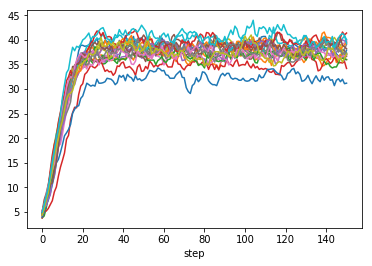
\includegraphics[width=0.8\textwidth]{scen_1_steady_state}
\caption{\% of Population Infected Over Time \\ Scenario 1}
\end{figure}


% minimum runs for statistically meaningful results

The average percentage of turtles infected at 50 ticks was 38.79. The sample standard deviation was 1.799, which indicates a margin of error at 95\% confidence of $\pm 0.842$ using a t-value of 2.093. This implies that to get a margin of confidence of 0.5, 56.7 trial runs would be required. When 56 trials were run, the result was $37.93 \pm 0.493$, so the estimate for $n$ was accurate. 

The total infection time per non-immune turtle per tick was also recorded. The 20 trial mean at tick 40 was $0.6343 \pm 0.00669$. This adjusts for turtle immunity and runtime in order to compare results across scenarios later on. 

% conclusions. 

Thus the model indicates that for these parameters, a fairly high number of turtles will contract the infection and the infection will be passed around continually rather than dying out at some point in the future. Considering the margin of errors for the results, if the model accurately reflects a real world scenario, we can have a good idea of how that scenario would play out. 

\subsubsection{Scenario 2}
%%%%%%%%%%%%%%%%%%%%
% describe

Scenario 2 looks at the flu in a society with high but imperfect immunization rates. In the US this is seen in cases where infants and the elderly cannot receive the vaccine and some people elect not to receive it or forget. This is accomplished by using the same recovery rate, 10\% but increasing immunity probability to 80\%. 


% time required to reach steady state

 Figure 3 shows the percentage of turtles infected over time. A steady state is more difficult to identify. The average percentage is lower than scenario 1 because of 80\% population immunity. The lower mean scales the y-axis of the chart down from 0-14 instead of 0-45 in scenario 1. Thus while the standard deviation looks higher it is essentially the same, 1.869 in scenario 1 and 1.853 in scenario 2. 

Because a steady state is less certain looking at the chart a t-test can be used to confirm that the mean of the set of trials is not changing between steps. At step 50 the mean percent infected was 5.92 with st. deviation 1.799. At step 100 these were 6.90 and 1.99. At step 250 7.935 and 1.696. At step 400 8.075 and 1.502. At step 500 7.956 and 2.113. 

The p-value for a t-test with the null hypothesis that the means at steps 50 and 100 are different was 0.116. Indicating a 12\% chance of different means and no steady state with 95\% confidence. The same test for the means at tick 250 and tick 500 had a p-value of 0.97. The test for steps 400 and 500 had a p-value of 0.84. Thus it is difficult to say with confidence that a steady state exists for this model as the effort to reject the null hypothesis that the means are different begins to resemble simply getting lucky enough to choose ticks with means that are very similar to each other by coincidence. 

Sicktime per turtle per tick at 100 ticks was $ 0.1047 \pm 0.01397$.

\begin{figure}
\centering
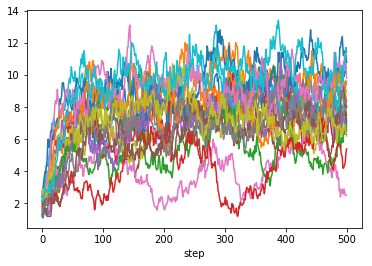
\includegraphics[width=0.8\textwidth]{20-runs-scenario-2-steady-state}
\caption{\% of Population Infected Over Time \\ Scenario 2}
\end{figure}


% minimum runs for statistically meaningful results

At tick 250, the mean percentage of turtles infected was $7.94 \pm 0.794$. the variability in results for this scenario is very similar to scenario 1 but that in light of the results of a t-test for a steady state, the true margin of error is likely to be higher since the process may not be stationary at tick 250, i.e. the true mean may change across ticks.  

\subsubsection{Scenario 3}

% describe

This scenario investigates the common cold using a higher rate of recovery 25\% and lower rate of immunity 5\% since there is no vaccine for the common cold and many members of society continue their daily routines with a cold exposing relatively more people than the flu. 

% time required to reach steady state

Figure 4 illustrates the percentage of turtles infected over time. Here a steady state seems more obvious. At 50 ticks the mean was 66.19 and st. deviation was 1.597. At 100 ticks this was 65.84 and 1.648. The 0.04994 p-value for a two tailed t-test indicates a 5\% probability of the null hypothesis that the means are different.

\begin{figure}
\centering
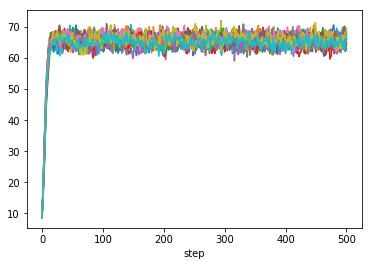
\includegraphics[width=0.8\textwidth]{20-runs-scenario-3-steady-state}
\caption{\% of Population Infected Over Time \\ Scenario 3}
\end{figure}

% minimum runs for statistically meaningful results

At 50 ticks the mean percentage of turtles infected was $66.08 \pm 0.902$ Results for sick time per turtle per tick at tick 50 were $0.311 \pm 0.0013$. Good margins of error in both cases. 


\subsection{Conclusion}

Comparing the three scenarios, The unvaccinated flu, scenario 1, resulted in a 38\% average infection rate while the vaccinated flu, scenario 2, resulted in 7.93\% of turtles infected on average. The common cold, scenario 3,  66\% of turtles infected. At tick 50, non-immune turtles in scenario 1 had spent 63\% of ticks infected on compared to 10\% in scenario 2 and 31\% in scenario 3, demonstrating the value of population immunity to non-immune members.  This model replicates the empirical idea of ``herd immunity''; general group immunity protecting non-immune members. 

To continue, one could test whether there is a constant increase in sick time per non-immune turtle or whether  sick time accelerates. One could also add  a parameter for infection contagiousness. Adding in death or post-infection immunity would be an interesting extension. 

%\textbf{1160 words}



\pagebreak

\section{Appendix 1}

\begin{verbatim}
#Recursive function for calculating node removal effects
  
node_deleter <- function(igraph_object, node_function, network_function, 
									depth, unconn) {

  # check that it's an igraph object
  if(class(igraph_object) != "igraph") {
    return("i_graph_object must be of class igraph")
  } else {
    
    # if igraph object is null (all nodes have been deleted) return null
    if(is.null(igraph_object)) {
      return(NULL)
    } else {
      
      # if depth == 0 return null if enough nodes have been deleted 
      # to complete the analysis
      if(depth == 0){
        
      } else {
        
        # match functions
        net_fun <- match.fun(network_function)
        node_fun <- match.fun(node_function)
        
        # calculate pre-deletion network measurement statistic 
        network_stat_1 = net_fun(igraph_object, unconnected = unconn)
        
        # call node_function on igraph object
        node_stats = node_stats_calc(igraph_object, fun = node_fun)
        
        # station_name = max station stat
        target <- node_stats[which.max(node_stats$stat),]
        target <- as.character(target[[1]])
        
        # delete station
        igraph_object = delete.vertices(igraph_object, c(target))
        
        #calculate post_deletion network statistic
        network_stat_2 = net_fun(igraph_object, unconnected = unconn)
        
        # calc change in network statistics due to deletion
        # a positive change means that trips have gotten longer
        network_change = network_stat_2 - network_stat_1
        
        # join deleted station name and effect
        value = data.frame(target, network_change, components(igraph_object)$no)
        
        # return value
        return (rbind(value, node_chopper(igraph_object, node_function, 
        	network_function, (depth - 1), unconn = unconn)))
        
      } 		# end deletion procedure
    } 			# end recurse check 
  } 			# end type check 
} 				# end function


\end{verbatim}

\nocite{*}


\printbibliography


\end{document}
